\documentclass[11pt]{report}
\usepackage[utf8]{inputenc}
\usepackage{geometry}
\usepackage{pdfpages}
\geometry{a4paper, top=1.25cm,bottom=1.5cm,right=1.5cm,left=1.5cm}
\usepackage{amsmath, amssymb, amstext}
\usepackage{tikz}
\usepackage{pgfplots}
\setlength\parindent{0pt}
\tikzset{myBound/.style={color=blue}}
\tikzset{myAxisLine/.style={line width=0.3mm,color=black}}
\tikzset{myLine/.style={thick,color=black}}
\usepackage{enumitem}
\usepackage{array}
\newcolumntype{M}{> {$} l < {$}}
\usepackage{mathtools}
\newcommand\Mycomb[2]{\prescript{#1\mkern-1mu}{}C_{#2 \mkern+6mu}}
\renewcommand{\baselinestretch}{1.2}
\usepackage{tkz-euclide}
\usetikzlibrary{positioning}

\definecolor{minGridCol}{RGB}{130, 255, 255}
\tikzset{myMajGrid/.style={color=gridCol, line width=0.0mm}}
\tikzset{myMinGrid/.style={color=minGridCol, line width=0mm}}
\tikzset{myAxisLine/.style={line width=0.3mm,color=black}}
\tikzset{myGraphPerm/.style={color=black,thick}}
\tikzset{myGraphPermGray/.style={color=black,ultra thin}}



\tikzset{myAngle/.style={thin,color=black}}
\newcommand\onelabel[6]{
	\tkzMarkAngle[myAngle,size =#1]({#2},{#3},{#4})
	\tkzLabelAngle[pos=#5 ]({#2},{#3},{#4}){\footnotesize ${#6}$}
}
\usepackage{titlesec}
\titleformat{\chapter}
%{\normalfont\huge\bfseries}{\chaptertitlename\ \thechapter}{20pt}{\Huge}   
%\titlespacing*{\chapter}{0pt}{-50pt}{40pt}
{\LARGE\bfseries}
{\chaptertitlename:~\thechapter \vspace{0cm}} {1em} {}
\titlespacing*{\chapter}{0pt}{0pt}{10pt}
\title{Properties of curves and applications of differentiation }
\author{Kh notes}
\date{}



%----------------------Triangles------------------------------------------
\newcommand{\x}{0}
\newcommand{\y}{0}
\newcommand\triangleSAS[7]{
	\renewcommand{\x}{0};
	\renewcommand{\y}{0};
	\coordinate (R) at (#5,#6);
	%\filldraw[red](\x,\y) circle [radius=1pt];
	%\filldraw[](0,0) circle[radius=1pt];
	\begin{scope}[ xshift=#5cm, yshift=#6cm,rotate around={#4:(R)}, scale around={#7:(R)} ]
		%\filldraw[blue](\x,\y) circle [radius=1pt];
		\coordinate(O) at(0,0);
		\coordinate(B) at (#3,0);
		\coordinate(A) at ({#1*cos(#2)},{#1*sin(#2)});		
	\end{scope}
	
}


%----------------------Bounding Boxes------------------------------------------
\newcommand\brect[2]{
	\draw[myBound](-#1,-#2)rectangle(#1,#2);
	%backcolour
	\draw[myBound, opacity=0.1, xstep=0.5cm, ystep=0.5cm](-#1,-#2)grid(#1,#2);
	\draw[myBound](0,0)circle[radius=2pt];
}
\begin{document}
	\maketitle
	\tableofcontents
	\newpage
	\chapter{Properties of curves}
\section{Review Questions}
\subsection{Some fundamental derivatives:}
\def\arraystretch{2}
\setlength\tabcolsep{1cm}
\newcommand{\sep}{0.25cm}
\begin{center}
	\begin{tabular}{| M | M |} \hline
		\text{Function} & \text{Derivative} \\\hline
		f(x)=x^n  & \displaystyle f'(x)=nx^{n-1}~~ (n \in \mathbb{R})\\ [\sep] \hline
		f(x)=e^x  & \displaystyle f'(x) =e^x\\ [\sep] \hline
		f(x)=\ln x  & \displaystyle f'(x) =\frac{1}{x}\\ [\sep] \hline
		f(x)=\sqrt{x}  & \displaystyle f'(x) =\frac{1}{2 \sqrt{x} }\\ [\sep] \hline
		f(x)=\sin{x}  & \displaystyle f'(x) =\cos{x}\\ [\sep] \hline
		f(x)=\cos{x}  & \displaystyle f'(x) =-\sin{x}\\ [\sep] \hline
		f(x)=\tan{x}  & \displaystyle f'(x) =\sec^2{x}\\ [\sep] \hline
	\end{tabular}
\end{center}
\subsection{Rules of differentiation:}
Chain Rule:
\begin{align*}
	y&= g(u_{(x)})\\
	\frac{dy}{dx} &= g'(u_{(x)} )u'_{(x)}
\end{align*}
Product Rule:
\begin{align*}
	y&= u_{(x)}v_{(x)}\\
	\frac{dy}{dx} &= u_{(x)}v'_{(x)} +u'_{(x)}v_{(x)}
\end{align*}
Quotient Rule:
\begin{align*}
	y&= \frac{u_{(x)}}{v_{(x)}}\\
	\frac{dy}{dx} &= \frac{ u'_{(x)}v_{(x)} - u_{(x)}v'_{(x)} }{ [ v_{(x)} ]^2 }
\end{align*}


\newpage
\section{Tangents}
\begin{itemize}
	\item The tangent to a curve at a point A is the best approximating straight line to the curve at point A.
	\item (Leibniz definition) Tangent to the curve $y=f(x)$ at the point $(a,f(a))$ is the line through the infinitely close pair of points either side of $f(a)$
	$$\frac{y-f(a)}{x-a} =\lim\limits_{h\to 0}\frac{f(a+h)-f(a)}{h}$$
	\item It is a single point of contact with the curve (although it may intersect the curve at some other point)
\end{itemize}\vspace{1cm}

\begin{center}
	

\begin{tikzpicture}[xscale= 0.6,yscale=0.6]
	%\draw[myMinGrid, xstep=1cm, ystep=1cm](-14,-5) grid(14,6);
	\draw[myAxisLine, <->](-14,0)--(14,0)node[right]{$x$};
	\draw[myAxisLine, <->](0,-5)--(0,7)node[above]{$y$};
	\draw[black](0,0) circle [radius=5pt];

\begin{scope}[yscale=1.5]
	\draw[yscale=1,xscale=1,domain=-11:10,smooth,variable=\x,blue, thick, <->] plot ({\x},{  -0.01*(\x+9)*(\x-9)*(\x+1)    });
		\renewcommand{\x}{7}
		\coordinate (A) at  (\x,0);
		\coordinate (A') at  (\x, {  -0.01*(\x+9)*(\x-9)*(\x+1)    } );
		\draw[dashed, red, thick](A)node[below]{$a$} -- (A');
		
				\renewcommand{\x}{7}
		\newcommand{\calc}{0};
		\renewcommand{\calc}{ -0.01*( 3*(\x)^2 +2*\x -81) };	
		\draw[yscale=1,xscale=1,domain=-3:3,smooth,variable=\t,red, thick] plot ( {\x+\t} ,{ -0.01*(\x+9)*(\x-9)*(\x+1) + \t*\calc    });
	
	\end{scope}
		\fill[red](A') circle [radius=4pt];
		\draw[](11,6)node[left]{$y=f(x)$};
\end{tikzpicture}\vspace{1cm}



\hrule\vspace{0.5cm}
For the function $y=f(x)$, and some $x=a$
\begin{itemize}
\item $(a,f(a))$ is on the curve 
\item $f'(a)$ is the gradient of the curve at $x=a$
\end{itemize}
\Large
\begin{alignat*}{2}
&&\frac{y-f(a)}{x-a}&=f'(a) \\
&\Rightarrow& y&= f'(a)(x-a) + f(a)
\end{alignat*}
\normalsize
Is the equation of the tangent line
\vspace{0.5cm}\hrule
\end{center}
\newpage
\subsection{Horizontal Tangents}
Horizontal tangents have a gradient of 0. \\
These will be very important later, when we investigate stationary points in more detail.\\\\


\begin{tikzpicture}[xscale= 0.6,yscale=0.6]
	%\draw[myMinGrid, xstep=1cm, ystep=1cm](-14,-5) grid(14,6);
	\draw[myAxisLine, <->](-14,0)--(14,0)node[right]{$x$};
	\draw[myAxisLine, <->](0,-5)--(0,7)node[above]{$y$};
	\draw[black](0,0) circle [radius=5pt];
	
	\begin{scope}[yscale=1.5]
		\draw[yscale=1,xscale=1,domain=-11:10,smooth,variable=\x,blue, thick, <->] plot ({\x},{  -0.01*(\x+9)*(\x-9)*(\x+1)    })node[below]{$y=f(x)$};
		\renewcommand{\x}{-5.54}
		\coordinate (A) at  (\x,0);
		\coordinate (A') at  (\x, {  -0.01*(\x+9)*(\x-9)*(\x+1)    } );
		\draw[dashed, red, thick](A)node[above]{$a$} -- (A');
			\draw[yscale=1,xscale=1,domain=-11:-1,smooth,variable=\t,red, thick] plot ({\t},{  -0.01*(\x+9)*(\x-9)*(\x+1)    })node[right]{$y=f(a)$};
		\renewcommand{\x}{4.873}
		\coordinate (B) at  (\x,0);
		\coordinate (B') at  (\x, {  -0.01*(\x+9)*(\x-9)*(\x+1)    } );
		\draw[dashed, red, thick](B)node[below]{$b$} -- (B');
			\draw[yscale=1,xscale=1,domain=1:8,smooth,variable=\t,red, thick] plot ({\t},{  -0.01*(\x+9)*(\x-9)*(\x+1)    }) node[right]{$y=f(b)$};
		
	\end{scope}
		\fill[red](A') circle [radius=4pt];
		\fill[red](B') circle [radius=4pt];

\end{tikzpicture}\vspace{1cm}

In general, we will need to find where the stationary points are:\\

\hrule\vspace{0.5cm}
\Large
\begin{itemize}
	\item Find $f'(x)$
	\item Solve $f'(x) = 0$
	\item Substitue the solution(s) into $f(x)$ to find the constant terms for the horizontal line equation
\end{itemize}
\normalsize
\vspace{0.5cm}\hrule


\newpage
\subsection{Ex13A}
\begin{itemize}
	\item Tangent equations from root and polynomial functions
	\item Horzontal tangents
	\item Natural log and exponent questions
	\item Concept questions 
\end{itemize}

\textbf{4 worked examples} 
\newpage
\includepdf[pages={1-},scale=0.85]{TangentQuestions.pdf} 
\newpage
\section{Normals}
\newcommand{\ang}{50}
\newcommand{\ext}{5}
The product of the gradients of perpedicular lines = -1\\
There are various proofs, one example below.\\
\begin{center}
\begin{tikzpicture}[xscale= 0.6,yscale=0.6]
	%\draw[myMinGrid, xstep=1cm, ystep=1cm](-14,-5) grid(14,6);
	\draw[myAxisLine, <->](-5,0)--(5,0)node[right]{$x$};
	\draw[myAxisLine, <->](0,-5)--(0,5)node[above]{$y$};
	%\draw[black](0,0) circle [radius=5pt];
	\draw[yscale=1,xscale=1,domain=-\ext:\ext,smooth,variable=\t,blue, thick] plot (  {\t*cos(\ang)},{ \t*sin(\ang)    });
	\draw[yscale=1,xscale=1,domain=-\ext:\ext,smooth,variable=\t,red, thick] plot (  {\t*cos(\ang + 90)},{ \t*sin(\ang + 90)    });
	\coordinate (O) at (0,0);
	\coordinate (A) at (  {\ext*cos(\ang)} ,{ \ext*sin(\ang)    });
	\coordinate (X) at ( {\ext*cos(\ang)} ,0);
	\coordinate (A') at (  {\ext*cos(\ang + 90)},{ \ext*sin(\ang +90)    });
	\coordinate (X') at ({\ext*cos(\ang + 90)},0);
	\onelabel{0.6}{X}{O}{A}{0.85}{\theta}
	
	\draw[dashed, blue](A) -- (X)node[midway, right]{\scriptsize $\sin(\theta)$};
	\draw[dashed, blue](O) -- (X)node[midway, above, xshift=0.3cm]{\scriptsize $\cos(\theta)$};
		\tkzMarkRightAngle[myLine,size=.4](A',O,A)
			\draw[dashed, red](A') -- (X')node[midway, left]{\scriptsize $\sin( \theta +\frac{ \pi }{2} )$};
		\draw[dashed, red](O) -- (X')node[midway, above, xshift=-0.1cm]{\scriptsize $\cos(\theta + \frac{ \pi }{2} )$};
		
		\draw[blue](8,4)node[right]{\Large $m=\frac{\sin(\theta)}{\cos(\theta)}$};
		\draw[red](8,2)node[right]{\Large $m_{\perp}=\frac{\sin(\theta +\frac{ \pi }{2} )}{\cos(\theta +\frac{ \pi }{2})}= - \frac{\cos(\theta)}{\sin(\theta)}$};
			\draw[black](8,0)node[right]{\Large $m \times m_{\perp} = -1$};
\end{tikzpicture}\vspace{1cm}

\hrule\vspace{0.5cm}
For the function $y=f(x)$, and some $x=a$
\begin{itemize}
	\item $(a,f(a))$ is on the curve 
	\item $\displaystyle -\frac{1}{f'(a)}$ is the gradient of the \textbf{normal to the curve} at $x=a$
\end{itemize}
\Large
\begin{alignat*}{2}
	&&\frac{y-f(a)}{x-a}&= -\frac{1}{f'(a)} \\
	&\Rightarrow& y&=  -\frac{1}{f'(a)}(x-a) + f(a)
\end{alignat*}
\normalsize
Is the equation of the tangent line
\vspace{0.5cm}\hrule\vspace{0.5cm}


\begin{tikzpicture}[xscale= 0.6,yscale=0.6]
	%\draw[myMinGrid, xstep=1cm, ystep=1cm](-14,-5) grid(14,6);
	\draw[myAxisLine, <->](-8,0)--(17,0)node[right]{$x$};
	\draw[myAxisLine, <->](0,-5)--(0,5)node[above]{$y$};
	\draw[black](0,0) circle [radius=5pt];
	\draw[yscale=1,xscale=1,domain=-8:11,smooth,variable=\x,blue, thick, <->] plot ({\x},{  0.01*(\x+9)*(\x-9)*(\x-1)    })node[left]{$y=f(x)$};
	%\draw[yscale=1,xscale=1,domain=-11:12,smooth,variable=\x,green, thick, dashed] plot ({\x},{  0.01*(3*(\x)^2 -2*\x -81)    });
	\draw[yscale=1,xscale=1,domain=3:12,smooth,variable=\x,red, thick] plot ({\x},{  0.52*\x -5.56   })node[right]{Tangent gradient = $f'(a)$};
	\draw[yscale=1,xscale=1,domain=4:9,smooth,variable=\x,teal, thick] plot ({\x},{ (-1/0.52)*\x + 11.542  })node[right]{Normal gradient = $-\frac{1}{f'(a)}$};

	
	\draw[black](7,-1.92) circle [radius=5pt];
	\draw[red ,dashed] (7,0)node[above]{$a$} -- (7,-1.92);

\end{tikzpicture}


\end{center}
\subsection{Ex 13B}
\newpage
\includepdf[pages={1-},scale=0.85]{NormalQuestions.pdf} 
\newpage
\section{Increasing and Decreasing}
When analysing functions, we are often interested in the intervals across which the function is  increasing or  decreasing.
\begin{itemize}
	\item If the gradient is entirely positive on an interval, the function is increasing on that interval.
	\item If the gradient is entirely negative on an interval, the function is decreasing on that interval.
\end{itemize}
If a function changes from increasing to decreasing, it must pass through a stationary point (or cross a region where the function is not differentiable)\\\\
Hnece we need to divide up the domain into intervals bounded by stationary points  and points where the function is not differentiable.\\
Finding a single gradient on each interval will tell us whether the function is increasing or decreasing.\\\\
We can communicate all of this using a \textbf{sign diagram}.




\subsection{Basic Sign Diagram example}

\begin{center}
	
	
	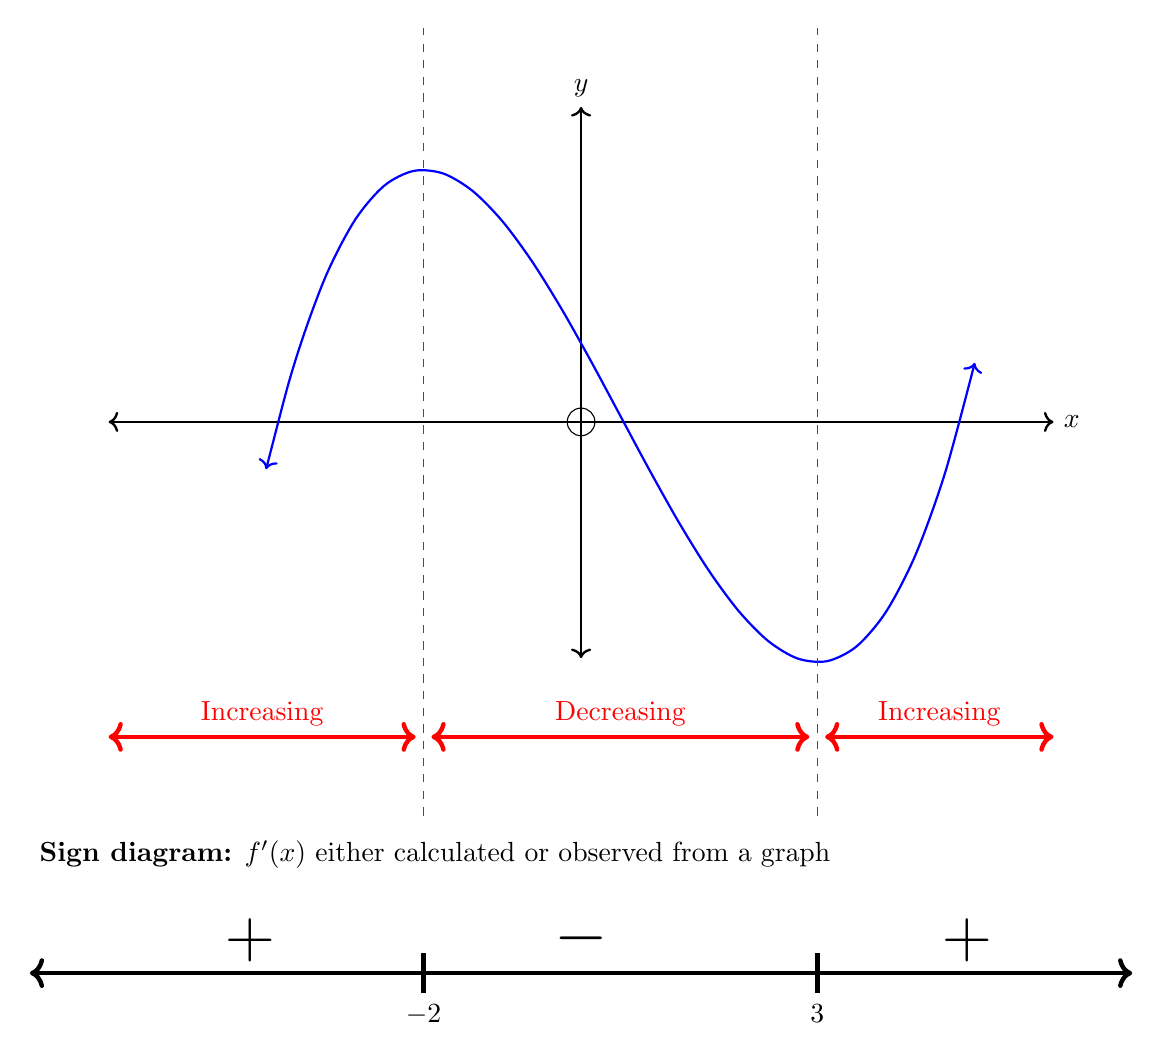
\begin{tikzpicture}[xscale= 1,yscale=1]
        %\draw[myMinGrid, xstep=1cm, ystep=1cm](-6,-5) grid(6,5);
		\draw[myAxisLine, <->](-6,0)--(6,0)node[right]{$x$};
		\draw[myAxisLine, <->](0,-3)--(0,4)node[above]{$y$};
		\draw[black](0,0) circle [radius=5pt];
		\draw[domain=-4:5,smooth,variable=\x,blue, thick, <->] plot ({\x},{ 0.1*\x^3  -0.15*((\x)^2)  -1.8*(\x) +1  });
			\renewcommand{\y}{-7}
			\renewcommand{\x}{-2}
			\newcommand{\shft}{3}
		\coordinate (A) at  (\x,-5);
		\coordinate (A') at  (\x,5);
		\draw[myAxisLine, ultra thick](\x,\y+0.25)--(\x,\y-0.25)node[below]{$-2$};
		\renewcommand{\x}{3}
		\coordinate (B) at  (\x,-5);
		\coordinate (B') at  (\x,5);
		\draw[red, dashed](A) -- (A');
		\draw[red, dashed](B) -- (B');
		\draw[myAxisLine, ultra thick](\x,\y+0.25)--(\x,\y-0.25)node[below]{$3$};
		\draw[myAxisLine, ultra thick, <->](-7,\y)--(7,\y)node[above, pos=0.2]{\Huge $+$ }node[above, pos=0.5]{\Huge $-$}node[above, pos=0.85]{\Huge $+$ };
		
		\draw[myAxisLine, red, ultra thick, <->](-1.9,\y+\shft)--(2.9,\y+\shft)node[midway, above]{Decreasing};
		\draw[myAxisLine, red, ultra thick, <->](-6,\y+\shft)--(-2.1,\y+\shft)node[midway, above]{Increasing};
		\draw[myAxisLine, red, ultra thick, <->](3.1,\y+\shft)--(6,\y+\shft)node[midway, above]{Increasing};
		
		\draw[](-7,-5.5)node[right]{\textbf{Sign diagram:} $f'(x)$ either calculated or observed from a graph };
		
	\end{tikzpicture}\vspace{1cm}
\end{center}

\newpage
\subsection{Sign Diagram example with discontinuites}
Below is the graph of $$y=\frac{x-3}{x^2-4}$$
Because division by 0 is undefined, the graph has vertical asymptotes when $x^2-4 =0$\\
(i.e when $x=2$ and $x=-2$ )\\\\
The derivative is $\displaystyle \frac{dy}{dx} = \frac{-x^2+6x-4}{(x^2-4)^2} $ and using a graphics calulator to solve $-x^2+6x-4=0$, \\\\
we have stationary points at $x\approx 0.764$ and $x\approx 5.236$\\\\


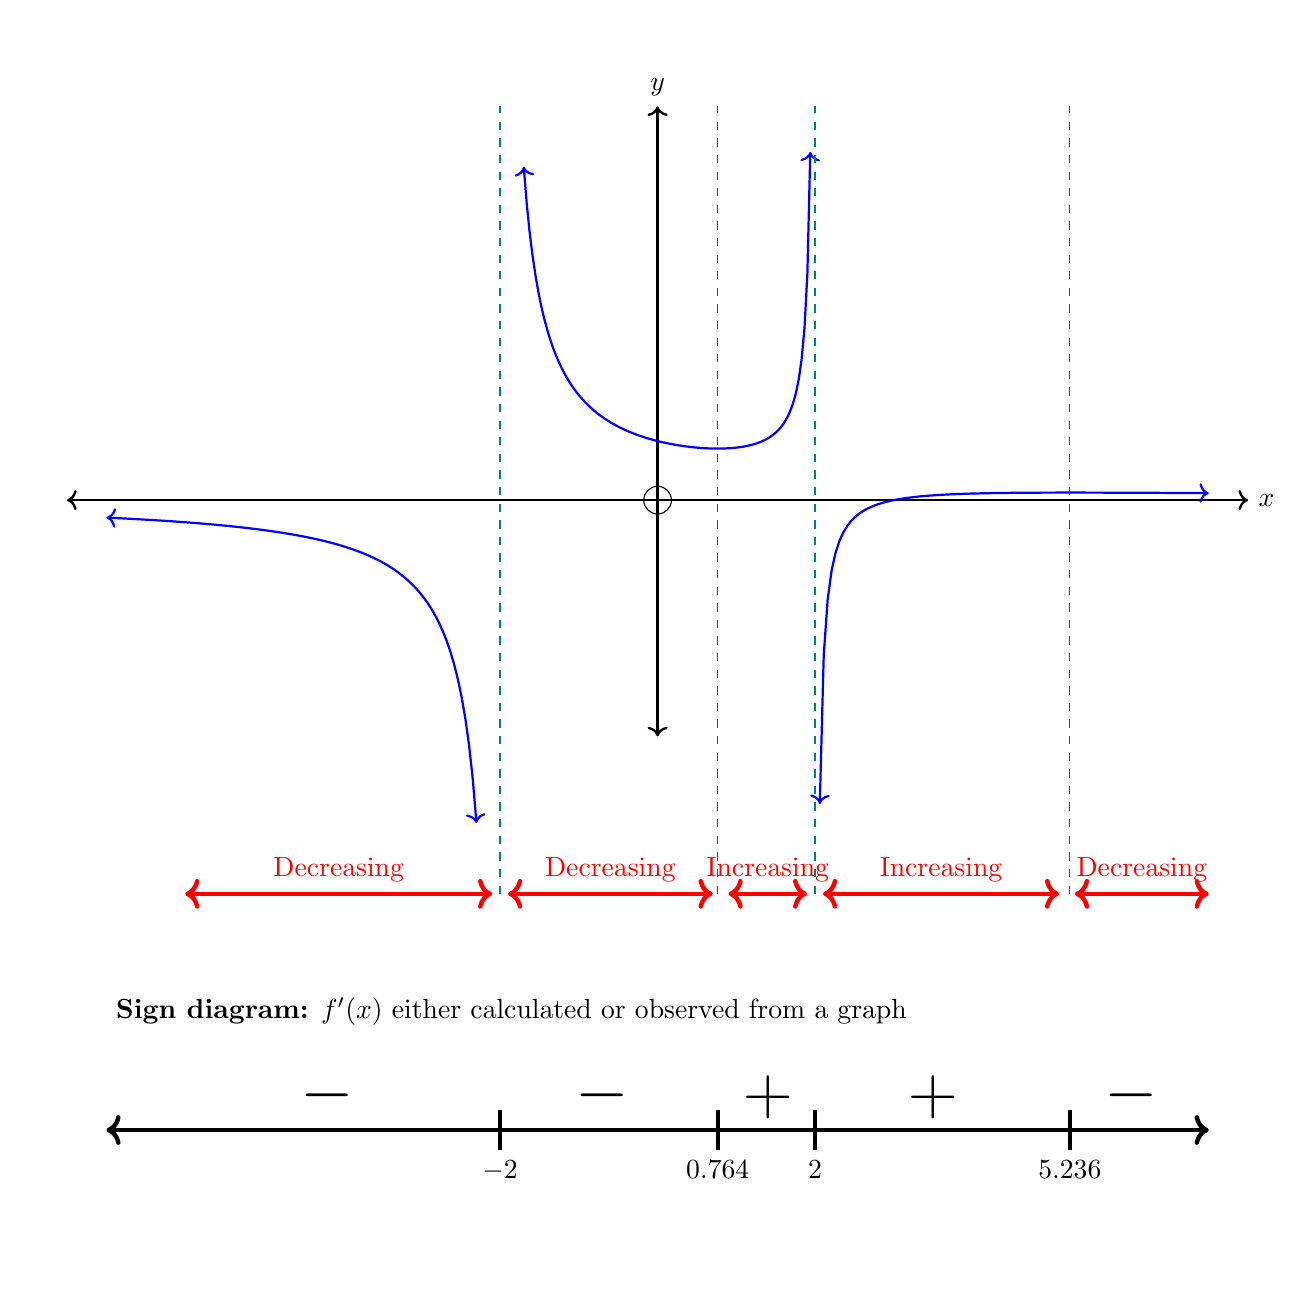
\begin{tikzpicture}[]
	 \clip(-8,-10) rectangle (8,6);
	%\draw[myMinGrid, xstep=1cm, ystep=1cm](-14,-5) grid(14,6);
	\draw[myAxisLine, <->](-7.5,0)--(7.5,0)node[right]{$x$};
	\draw[myAxisLine, <->](0,-3)--(0,5)node[above]{$y$};
	\draw[black](0,0) circle [radius=5pt];
	

		\draw[yscale=1,xscale=1,domain=-1.7:1.94, samples=100,variable=\x,blue, thick, <->] plot ({\x},{  (\x-3)/((\x)^2-4)   });
		\draw[yscale=1,xscale=1,domain=-7:-2.3, samples=100,variable=\x,blue, thick, <->] plot ({\x},{  (\x-3)/((\x)^2-4)   });
		\draw[yscale=1,xscale=1,domain=2.06:7, samples=100,variable=\x,blue, thick, <->] plot ({\x},{  (\x-3)/((\x)^2-4)   });
		\renewcommand{\y}{-8}
		\renewcommand{\x}{-2}
		\coordinate (A) at  (\x,-5);
		\coordinate (A') at  (\x,5);
		\draw[dashed, teal, thick](A) -- (A');
		\draw[myAxisLine, ultra thick](\x,\y+0.25)--(\x,\y-0.25)node[below]{$-2$};
		\renewcommand{\x}{2}
		\coordinate (B) at  (\x,-5);
		\coordinate (B') at  (\x, 5 );
		\draw[dashed, teal, thick](B) -- (B');
		\draw[myAxisLine, ultra thick](\x,\y+0.25)--(\x,\y-0.25)node[below]{$2$};
		
	
		\renewcommand{\x}{0.764}
		\newcommand{\shft}{3}
		\coordinate (C) at  (\x,-5);
		\coordinate (C') at  (\x,5);
		\draw[myAxisLine, ultra thick](\x,\y+0.25)--(\x,\y-0.25)node[below]{$0.764$};
		\renewcommand{\x}{ 5.236}
		\coordinate (D) at  (\x,-5);
		\coordinate (D') at  (\x,5);
		\draw[red, dashed](C) -- (C');
		\draw[red, dashed](D) -- (D');
		\draw[myAxisLine, ultra thick](\x,\y+0.25)--(\x,\y-0.25)node[below]{$5.236$};
		\draw[myAxisLine, ultra thick, <->](-7,\y)--(7,\y)node[above, pos=0.2]{\Huge $-$ }node[above, pos=0.45]{\Huge $-$}node[above, pos=0.6]{\Huge $+$ }node[above, pos=0.75]{\Huge $+$ }node[above, pos=0.93]{\Huge $-$ };
		
		\draw[myAxisLine, red, ultra thick, <->](-6,\y+\shft)--(-2.1,\y+\shft)node[midway, above]{Decreasing};
		\draw[myAxisLine, red, ultra thick, <->](-1.9,\y+\shft)--(0.7,\y+\shft)node[midway, above]{Decreasing};
		\draw[myAxisLine, red, ultra thick, <->](0.9,\y+\shft)--(1.9,\y+\shft)node[midway, above]{Increasing};
		\draw[myAxisLine, red, ultra thick, <->](2.1,\y+\shft)--(5.1,\y+\shft)node[midway, above]{Increasing};
		\draw[myAxisLine, red, ultra thick, <->](5.3,\y+\shft)--(7,\y+\shft)node[midway, above]{Decreasing};
		
		\draw[](-7,-6.5)node[right]{\textbf{Sign diagram:} $f'(x)$ either calculated or observed from a graph };
		\draw[blue](10,5)node[right]{$y=f(x)$};

		


	
\end{tikzpicture}\vspace{1cm}
\section{Stationary Points}
\subsection{Turning points (minima, maxima)}
\subsection{Stationary points of inflection}
\section{Shape}
\section{Inflection Points}
\section{Understanding functions and their derivatives}

\chapter{Applications of differentiation}







\newpage
% I prefer the alignment at the equal sign.
\begin{alignat*}{2}
	&\text{The equation is:}\qquad & 9a-4 &= 14+3a\\
	&\text{Subtract $3a$:} & 6a-4 &= 14\\
	&\text{Subtract 4:} & 6a &= 18\\
	&\text{Divide by 6:} & a &= 3
\end{alignat*}

$$A\widehat{B}C$$
$$A\widehat{BC}C$$
$$A\hat{B}C$$
$$N \tilde{a}$$
$$X \sim \mathcal{N}(\mu,\,\sigma^{2})$$

\newpage

\begin{center}
	\begin{tikzpicture}[scale=0.75]
		\draw[myBound](0,-0.5)rectangle(16,8);
		\begin{axis}[
			scale only axis,
			width=16cm, 
			height=8cm,
			restrict y to domain = 0:100,
			axis line style=ultra thick, axis x line=center,axis y line=center,ymajorgrids,yminorgrids,
			minor y tick num=0, xmajorgrids, xminorgrids, minor x tick num=0,major grid style=white, minor grid style=myMinGrid, xtick={-4,-3.5,...,3.5}, ytick={-4,-3,...,6},
			xlabel={$t$}, ylabel={$s(t)$}, xlabel style={below right}, ylabel style={above}, xmin=-4.5, xmax=4, ymin=-5, ymax=7]
			\addplot [myGraphPerm, domain=-6:6, smooth] { (x-3)/((x^2) -4) };
			\addplot [myGraphPermGray, domain=-4:0, smooth,dashed] {3*x^3-2*x^2-5*x};
			\addplot[] coordinates {(2,-1)}node[right]{$s(t)=3t^3-2t^2-5t$ };
		\end{axis}
\end{tikzpicture}\end{center}\normalsize

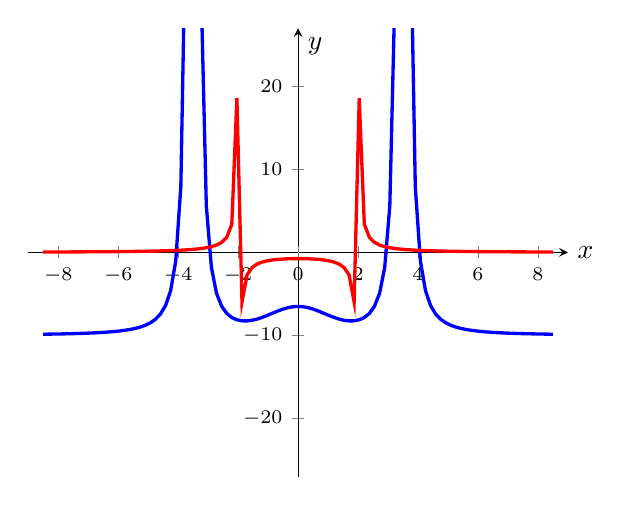
\begin{tikzpicture}
	\begin{axis}[
		axis lines=center,
		xlabel = {$x$}, xlabel style = {anchor=west},
		ylabel = {$y$},
		xmin=-9, xmax=9, xtick={-8,-6,...,8},
		extra  x ticks = {0},
		ymin=-27,  ymax=27,
		tick label style = {font=\scriptsize},
		domain = -8.5:8.5,
		restrict y to domain = -1000:1000,
		no marks,
		every axis plot post/.append style={very thick},
		]
		\addplot +[samples=101]
		{(3)/(x+3.5)^2 + (3)/(3.5-x)^2 + 3*e^(-((0-x)^2)/(2 * 1^2)) - 10};
		\addplot +[samples=101]
		{(3)/(x^2 - 4)};
	\end{axis}
\end{tikzpicture}









\end{document}